\section{Risk management}
\label{chap:risk_management}
According to IBM \parencite{IBM_risk_management}, risk management is the process of identifying, assessing and controlling the risks to an organisation's capital and earnings: these risks could arise from different sources, including accidents, malicious attacks and natural disasters.

The impact of unforeseen negative events could be catastrophic and have significant consequence on (the assets of) your organisation.
Therefore, a proper approach to risk management can help identify, manage and mitigate risks.
The three fundamental steps (i.e., risk identification, risk analysis and assessment and risk mitigation and monitoring) of the risk management process are described below.

Risk identification is the process of identifying and assessing threats (e.g., assessing IT security threats such as malwares and malicious attacks).

Risk analysis consists of establishing the probability of occurence of each risk and the potential outcomes of each negative event.

Risk assessment evaluates each risk, comparing the magnitude of each of them and ranking them with reference to their significance and consequences.

Risk mitigation is the process of planning and developing methods and options to limit threats to your organisation objectives.
Since this is a continuous process that evolves over time, risk monitoring can help in the coverage of known and unknown risks.

Moreover, there are five commonly accepted strategies for addressing risk:
\begin{itemize}
    \item risk avoidance: mitigating the risk by avoiding activities that may negatively affect the organisation;
    \item risk reduction: accepting the risk, minimising its consequences (i.e., focusing on keeping the loss contained, preventing it from spreading);
    \item risk sharing: transferring the possibility of loss from the individual to the group;
    \item transferring risk: contractually transferring a risk to a third-party (e.g., insurance shifts the risk from the organisation to the insurance company);
    \item risk acceptance and retention: since it is virtually impossible to eliminate all risk (except by totally avoiding it), some risk will remain (i.e., residual risk).
\end{itemize}


\subsection{Information security investments}
Usually, information security investments compete for resources (e.g., budget) with other investment opportunities. Though, the financial decision makers should choose how to allocate financial resources and which investments to carry out.
Although investing in new equipment or infrastructure to support an alternative business opportunity could seem profitable, the impact of possibly successful cyber attacks should be taken in consideration: the benefits of these investments could be made irrelevant by a successful attack \parencite{Conrad}.

As for any organisation, security managers need to measure their investments' cost-effectiveness, thus justifying their budget usage and providing arguments for their next budget claim.
However, since security is an investment that tipically provides loss prevention rather than direct profit \parencite{ENISA}, measuring the effectiveness and the cost of information security activities is often difficult.

Among the financial metrics used to estimate risks, there is the ALE (Average Loss Expectancy), calculated as the sum of the products of annual consequences and frequencies of occurrence \parencite{NBS}.
Since ALE dangerously equates likely but low impact events with unlikely but high impact events and since ALE-based risk models become overly complex when used to address all threats, assets and vulnerabilities, security risk measures require more robust approaches in identifying the true potential of threat exposure \parencite{Sectara}: the usage of a stochastic approach (e.g., Monte Carlo Method) to evaluate risks is recommended \parencite{Soo_Hoo}.

\subsection{Monte Carlo Simulation}
Monte Carlo Simulation (also known as the Monte Carlo Method) is a mathematical technique used to estimate the possible outcomes of an uncertain event: it predicts a set of outcomes based on an estimated range of values (instead of fixed input values, like other forecasting methods).

A Monte Carlo Simulation builds a model of the possible outcomes by exploiting a probability distribution, for any variable that has inherent uncertainty and it, then, recomputes the results multiple times, each time using a different set of random numbers within the bounds: as the number of inputs increase, the number of forecast also grows, allowing you to project outcomes farther out in time with more accuracy.
Upon the completion of a Monte Carlo Simulation, a range of possible outcomes with the respective probability of occurence is carried out.

The Monte Carlo techniques involves three basic steps:
\begin{enumerate}
    \item set up the predictive model, identifying both the dependent variables to be predicted and the independent variables that will drive the prediction;
    \item specify the probability distributions of the independent variables identified at step 1;
    \item run simulations repeatedly, generating random values of the independent variables, until enough results are gathered to make up a representative sample of the possible combinations.
\end{enumerate}

\subsection{Monte Carlo Simulation as a risk management tool}
Using a Monte Carlo Method-based approach in the analysis of information security investments is effective in evaluating the return on investments that defend against security attacks.
This approach captures uncertainty in security modeling parameters (e.g., vulnerabilities, frequency of instrusion, damage estimates) and expresses its impact on the model's forecast (e.g., projected benefit).

In a Monte Carlo Simulation, the security model is treated as a function that takes a set of parameters and returns a set of (forecasted) result, as can be seen in figure \ref{fig:simulation}.

\begin{wrapfigure}{l}{0.5\textwidth}
\centering
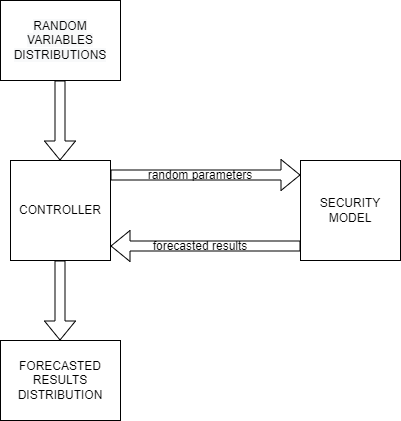
\includegraphics[width=0.8\linewidth]{Resources/mcs.png}
\caption{Schema of the Monte Carlo Simulation model}
\label{fig:simulation}
\end{wrapfigure}

More precisely:
\begin{enumerate}
    \item a set of random variables are identified (they represent the expert's estimates);
    \item a probability distribution is specified for each of the random variables identified at step 1 (the distributions represent the expert's estimates);
    \item a random value for each parameter, sampled according the distribution associated to the respective random variable, is given to the security model (i.e., selection);
    \item the security model is executed within the values passed as parameters (i.e., execution);
    \item the (forecasted) results are collected (i.e., collection).
\end{enumerate}

Naturally, selection, execution and collection phases are repeated in many iterations (usually thousands) of the security model.

Before building a simulation, it is fundamental to ensure that each iteration of the simulation is supplied with independent parameters (i.e., the input random variables must be independent) in order to carry out meaningful results.


\subsection{A case study}
Monte Carlo Simulation model can be used within the context of IT to reduce the disparities of opinion in resource allocation (e.g., allocating optimal resources to specific security protective assets or other business productive assets).

A Monte Carlo Simulation can perform quantitative risk analysis by assigning a probability distribution to uncertain parameters and through random sampling of the distribution: thus, it is possible to determine all potential outcomes under those uncertainties \parencite{Vose}.

Using a conceptual enterprise as a case study and verifiable historical cost of security breaches as parametric values, the model described shows why using conventional risk assessment approach as budgeting process can result in significant over/under allocation of resources for cyber capabilities.

\subsubsection{Overview}
Traditionally, organisations use risk assessment models to determine the optimal allocation of resources to cyber capabilities.
Then, financial decisions are based on the organisation's threat tolerance and its score from the risk scoring matrix.

The risk scoring matrix is calculated on the assumption that an event will happen given a probability of occurrence and a measure of the impact or severity of an associated security breach.
Information security budget is then allocated based on the resultant estimated risk score.

According to the risk scoring formula, the risk \textit{R} associated to an asset is given as the product of the probability \textit{P} of occurence of possibly negative events and the impact \textit{I} of these latters on the given asset, namely: \begin{equation} R = P * I \end{equation}
The values of \textit{P} and \textit{I} for a given asset is assigned based on security experts' opinions, statistic from reports, corporate level assessments or records from past events and the resultant single value represents the risk score \textit{R} for that particular asset.

In practice, in real word problems, it is difficult to follow this approach in order to optimise resource allocation decisions: the deterministic estimates carried out might not reflect the actual organisation's context.
Furthermore, a risk-matrix based approach may lead security assessors to assume that (under some assumptions) certain events would be true while completely ignoring the possible occurence of least significant events.

Hence, in order to explain how uncertainty affects security breach costs and resource allocation decisions to mitigate those risks, a case study is analysed below.

The scenario presented \parencite{Fagade} refers to a bank and the following assumptions are made:
\begin{itemize}
    \item there are five key assets (namely, DDoS Mitigation System, Personnel and third party contractors, Data Backup and Recovery System, Incident Response Solution, and Antivirus Software) that need to be safeguarded from security threats;
    \item resource allocation decisions are based on the impact of breaches to those assets and how they may impact banking operations.
\end{itemize}

Therefore, security breach costs estimation approaches are described below.

\subsubsection{Deterministic estimation of security breach costs}
This approach is based on the use of a conventional risk assessment models to determine appropriate resource allocation.

Each risk is ranked within a five level scale of likelihood and a scale of (financial) impact, as shown in tables \ref{tab:likelihood} and \ref{tab:severity}.

\begin{table}[H]
    \centering
    \begin{tabular}{|p{2cm}|p{6.5cm}|p{5cm}|}
         \hline
         \textsc{Likelihood} & \textsc{Description} & \textsc{Frequency of occurrences} \\
         \hline
         1 & An incident is expected to occur in exceptional circumstances (e.g., once in 10 years) & Rare/Very Low \\
         \hline
         2 & An incident may occur at some point (e.g., once in 3 years) & Possible/Low \\
         \hline
         3 & An incident will occasionally recur (e.g., once in a year) & Probable/Medium \\
         \hline
         4 & An incident will occur in most circumstances (e.g., once every 4 months) & Certain/High \\
         \hline
         5 & An incident is certain to occur in most circumstances (e.g., once every month) & Frequent/Very High \\
         \hline
    \end{tabular}
    \caption{Risk likelihood}
    \label{tab:likelihood}
\end{table}

\begin{table}[H]
    \centering
    \begin{tabular}{|p{2cm}|p{5.5cm}|p{6cm}|}
        \hline
        \textsc{Severity} & \textsc{Description} & \textsc{Example of business impact} \\
        \hline
        1 & None: no disruption of service & Financial loss $<$ 1000€ \\
        \hline
        2 & Minor & Financial loss $<$ 10'000€ \\
        \hline
        5 & Moderate & Financial loss $<$ 100'000€ \\
        \hline
        10 & Significant & Financial loss $<$ 1'000'000€ \\
        \hline
        15 & High & Financial loss $>$ 1'000'000€ \\
        \hline
    \end{tabular}
    \caption{Risk severity}
    \label{tab:severity}
\end{table}

With reference to the risk scoring formula yet presented, the risk scoring matrix can be computed by taking into account the likelihood and severity values of each risk.
In practice, risk scoring is carried out by multiplying the likelihood of each risk by the severity of that risk occurring.

\begin{table}[H]
    \centering
    \begin{tabular}{|c|c|c|c|c|c|}
        \hline
        \textsc{Likelihood / Severity} & \textsc{None} & \textsc{Minor} & \textsc{Moderate} & \textsc{Significant} & \textsc{High} \\
        \hline
        \textsc{Frequent} & \cellcolor{yellow} 5 & \cellcolor{yellow} 10 & \cellcolor{orange} 25 & \cellcolor{red} 50 & \cellcolor{red} 75 \\
        \hline
        \textsc{Certain} & \cellcolor{green} 4 & \cellcolor{yellow} 8 & \cellcolor{orange} 20 & \cellcolor{red} 40 & \cellcolor{red} 60 \\
        \hline
        \textsc{Probable} & \cellcolor{green} 3 & \cellcolor{yellow} 6 & \cellcolor{orange} 15 & \cellcolor{orange} 30 & \cellcolor{red} 45 \\
        \hline
        \textsc{Possible} & \cellcolor{green} 2 & \cellcolor{green} 4 & \cellcolor{yellow} 10 & \cellcolor{orange} 20 & \cellcolor{orange} 30 \\
        \hline
        \textsc{Rare} & \cellcolor{green} 1 & \cellcolor{green} 2 & \cellcolor{yellow} 5 & \cellcolor{yellow} 10 & \cellcolor{orange} 15 \\
        \hline
    \end{tabular}
    \caption{Risk scoring matrix}
    \label{tab:scoring}
\end{table}

After the risk analysis phase, given an organisation risk threshold and the risk score number, the budget is allocated for countermeasures to mitigate risks in that context.


\subsubsection{Probabilistic estimation of security breach costs}
As the assets grow, probabilistic estimation approaches can be used in place of conventional deterministic ones, in order to address the huge amount of uncertainties associated with these latter.

Using Monte Carlo Method, the probabilistic costs of security breaches for each asset in a given scenario can be determined.
In fact, a Monte Carlo Simulation works by sampling several scenarios from a probability distribution instead of static estimates (e.g., like in the deterministic approach just described). 
Probabilistic estimation assigns minimum and maximum cost boundaries for each security breach.
The combined cost of all security breaches is then calculated as the total minimum and maximum cost of a security breach for each asset in order to project total resource allocation for the enterprise.
In that case, it is possible to establish absolute bounds for allocated resources to the entire enterprise. 
Monte Carlo may not be able to tell with certainty the exact cost of a breach, but it can describe the probability of cost associated with security breaches, to aid resource allocation. 
In comparison to the deterministic approach, the probabilistic estimate is also based on random variables, however, each estimate follows a particular distribution, independent and unaffected by other variables.

\begin{table}[H]
    \centering
    \begin{tabular}{|p{6cm}|p{5cm}|p{4cm}|}
        \hline
        \textsc{Asset} & \textsc{Security incident} & \textsc{\textit{C} = Cost of breach} \\
        \hline
        DDos Mitigation System & DoS/DDoS attack & 53'477€ \\
        \hline
        Personnel and third party contractors & Fraud, malicious insider & 40'403€ \\
        \hline
        Recovery System & Data loss, stolen devices & 39'905€ \\
        \hline
        Incident Response Solution & Cyber espionage & 69'026€ \\
        \hline
        Antivirus Software & Malicious code infection & 31'572€ \\
        \hline
    \end{tabular}
    \caption{Expert estimation of security breach costs}
    \label{tab:expert_estimation}
\end{table}

Consider the deterministic cost of breach for the DDoS Mitigation System as described in table \ref{tab:expert_estimation}.
Under probabilistic estimation approach, \textit{blurring} parameter can be used to suggest that in place of a fixed quantity like 53'477€, the minimum value in of 30'000€ and the maximum value of 65'000€ in a distribution could be included, as shown in table \ref{tab:simulation_parameters}.
Essentially, a fixed value is replaced with a probability distribution, which is a true representation of the state in the real world.
Hence, the fixed quantity is now our most likely value, but it is not the only possible value in the distribution.
The key to Monte Carlo simulation is that each variable is assigned a random value, and the total value is calculated thousands of times during the simulation.
It, therefore, allows us to understand the risk that expectations may not match reality, hence, appropriate precautions can be taken \parencite{RiskAMP}.

\begin{table}[H]
    \centering
    \begin{tabular}{|p{6cm}|p{4cm}|p{1.3cm}|p{1.3cm}|p{1.3cm}|}
        \hline
        \textsc{Asset} & \textsc{Security incident} & \textsc{\textit{C\textsubscript{min}}} & \textsc{\textit{C\textsubscript{ml}}} & \textsc{\textit{C\textsubscript{max}}} \\
        \hline
        DDos Mitigation System & DoS/DDoS attack & 30'000€ & 53'477€ & 65'000€ \\
        \hline
        Personnel and third party contractors & Fraud, malicious insider & 20'000€ & 40'403€ & 50'000€ \\
        \hline
        Recovery System & Data loss, stolen devices & 25'000€ & 39'905€ & 45'000€ \\
        \hline
        Incident Response Solution & Cyber espionage & 35'000€ & 69'026€ & 75'000€ \\
        \hline
        Antivirus Software & Malicious code infection & 15'000€ & 31'572€ & 37'000€ \\
        \hline
        Total & & 123'000€ & 234'383€ & 272'000€ \\
        \hline
    \end{tabular}
    \caption{Model simulation parameters}
    \label{tab:simulation_parameters}
\end{table}

It is difficult to compute values for multiple scenarios without some form of simulation, especially if factoring in multiple assets and security breach costs, as part of the budgetary allocation process, is needed.

\subsection{Setup}
There are two basic assumptions for this model:
\begin{itemize}
    \item Key information asset points are determined by an organisation CIO and the security team;
    \item Minimum and maximum values of security breach costs are subject to expert elicitation, based on experience and previous security breach events.
\end{itemize}

The work described in this paper use some security breach cost parametric values obtained from verifiable information security breach reports \parencite{Ponemon} and \parencite{Kaspersky}.
Please note that limitations of the costing methodology outlined in these latter are not validated nor described neither in this paper nor in Fagade et al.'s one \parencite{Fagade}.

Before starting the simulation, security breach costs are identified and converted into a range of values using a probability distribution (i.e., for each security breach cost estimate, fixed values are replaced with a probability distribution).

Since the triangular distribution is one of the most used probability distributions to draw out expert opinion (especially in the case of limited or absence of historical data), the latter is used in this simulation.
The triangular distribution defines, for each asset, uncertain security breach cost values as a minimum \textsc{\textit{C\textsubscript{min}}}, maximum \textsc{\textit{C\textsubscript{max}}} and most-likely \textsc{\textit{C\textsubscript{ml}}} range of values.

Here, actually, the approach followed holds \textsc{\textit{C\textsubscript{min}}} and \textsc{\textit{C\textsubscript{max}}} constant while randomly selecting \textsc{\textit{C\textsubscript{ml}}} according to a triangular distribution.

For this simulation, MATLAB \parencite{MATLAB} and Vose ModelRisk software \parencite{ModelRisk} are used: both tools allow configurable simulations with a very large number of runs and can generate thousands of scenarios for each set of uncertain inputs.

The simulation runs generated are 50'000, the model output is a probabilistic range of values and scenarios associated with security breach costs, as well as the probability distribution associated with those values.

\subsection{Simulation results}
Results of Monte Carlo Simulation are shown in figures  \ref{fig:MR_results} and  \ref{fig:ML_results} and discussed, as reported in Fagade et al.'s paper \parencite{Fagade}, below.

For each iteration, the following steps are performed:
\begin{enumerate}
    \item samples are taken from each of the breach cost (triangular) probability distribution;
    \item the average random value (i.e., the total probabilistic estimation of security breach) is computed, at the end of the current iteration.
\end{enumerate}
At the end of the simulation (here, 50'000 iterations are run), the output histogram represents the generated scenarios (during the simulation, different scenarios are generated asccording to the probability of those scenarios occurring) for security breach cost.

\begin{figure}[H]
\begin{minipage}{.5\textwidth}
  \centering
  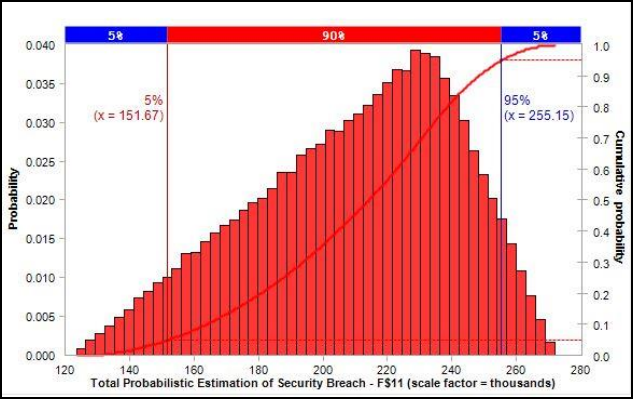
\includegraphics[width=1\linewidth]{Resources/ModelRisk_results.png}
    \captionof{figure}{Simulation results in ModelRisk}
    \label{fig:MR_results}
\end{minipage}%
\begin{minipage}{.5\textwidth}
  \centering
  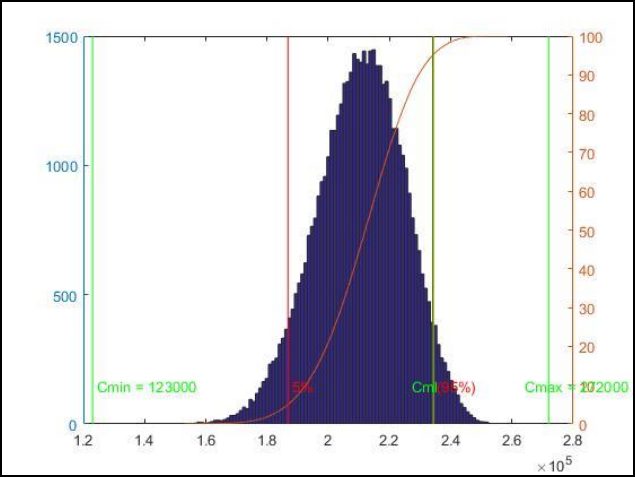
\includegraphics[width=1\linewidth, height=5.35cm]{Resources/MATLAB_results.png}
    \captionof{figure}{Simulation results in MATLAB}
    \label{fig:ML_results}
\end{minipage}
\end{figure}

From the simulation results in figure \ref{fig:MR_results}, it can be seen that the upper 5\% and the lower 5\% represent extreme cases that are ignored by the simulation output.

From the model simulation parameters in table \ref{tab:simulation_parameters}, it can be seen that the total resource allocation could be within the range of 123'000€ and 272'000€, but the realistic chance of resource allocation nearing these extreme values is very unlikely, hence the model ignored them.

Furthermore, it can be seen that 90\% of the simulation iterations fall under a value less than the upper bound estimated total values: hence, we can say that 90\% of the total allocation will meet the initial estimate (this is not a guarantee, but it allows us to adjust IT security budget to match the cost of potential breaches and also understand the risk that resource allocation may not meet initial estimates).

Further analysis of the result in figure \ref{fig:MR_results} shows that, given all the iterations of the simulation, the absolute minimum value of 149'794€ is much higher than the original deterministic lower bound value of 123'000€.

Similarly, the absolute maximum probabilistic value of 253'000€, after iterations, is much lower than the deterministic value of 272'000€ (with only 5\% chance of the allocation going over the upper boundary). 

The most likely point estimate is around the value of 290'000€; from the location of the peak of the distribution, it can be seen that this value is rather more realistic than the deterministic value of 234'383€ (this does not rule out the possibility that the cost of impact could be significantly higher, possibly twice as high in terms of cumulative percentage). 

Now, results are compared with another simulation in MATLAB, as shown in figure \ref{fig:ML_results}, using the same input parametric values.

The invariant that holds in both states of the models is that extreme values are ignored in the output of both simulations.
While both models follow a similar distribution, it can be seen that not only did both simulations ignore lower and upper bound values, but also shows higher \textsc{\textit{C\textsubscript{min}}} and lower \textsc{\textit{C\textsubscript{max}}} than the 
deterministic values.
